\documentclass[a4paper,11pt]{report}
\usepackage[]{amsmath}
\usepackage[]{physics} % \bra, \ket etc
\usepackage{graphicx} %Pour les figures je crois
\usepackage{hyperref}
\usepackage[
    backend=biber, 
    natbib=true,
    style=numeric,
    sorting=none, %Pour faire apparaitre les refs dans l'ordre
    hyperref=true
]{biblatex} %Imports biblatex package
\addbibresource{Bib_ch4.bib} %Import the bibliography file

\usepackage{amssymb} %quelques symboles dont gtrsim /lesssim
\usepackage{subcaption} % package pour faire des subfigures
\usepackage{multirow} % package pour multirow/multicolumn
\usepackage{booktabs} % package pour top/mid/bottom rule
\usepackage{tcolorbox} % toujours plus de boites
\usepackage{xcolor} % Pour avoir des couleurs dans les équations

\title{}
\begin{document}
\chapter{Influence of the magnetic field misalignment and laser polarization on the low field relaxation}

\section{Magnetic field alignment}
\begin{figure}[h]
\centering
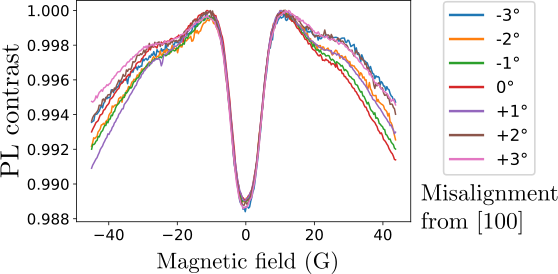
\includegraphics[width=.7\textwidth]{Figures/alignement_rose}
\caption{PL of sample CVD-pink as a function of the magnetic field for 7 different misalignment of the field with respect to the [100] axis}
\label{alignement rose}
\end{figure}

A potential cause for the observation of depolarization at low magnetic field when $\mathbf{B} \parallel [100]$ could be a misalignment of the magnetic field with the [100] axis. Indeed, such a misalignment would cause a splitting of the 4 classes as the magnetic field increases which would reduce the inter-class flip-flop rate. %This hypothesis is not consistent with the observations in Fig. \ref{scan 100}-d): we would expect a small  misalignment to cause a slow but steady decrease of $1/T_1^{\rm dd}$ as the magnetic field is increased. Instead we observe a sharp decrease followed by a pseudo-plateau.
Fig. \ref{alignement rose} shows the PL of sample CVD-pink as the magnetic field is scanned with various misalignments compared to the [100] axis. We estimate our alignments to be precise within $\pm 1^\circ$. We can see that the central feature is almost unaffected by the orientation within [$-3^\circ$:$+3^\circ$] which confirms that the low field depolarization in the $\mathbf{B} \parallel [100]$ case does not come from a field misalignment.

\section{Laser polarization}
\begin{figure}[h]
\centering
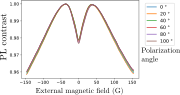
\includegraphics[width=.7\textwidth]{Figures/pola_laser}
\caption{PL of sample ADM-150-3 as a function of the magnetic field for six different laser polarization angles. The magnetic field orientation was chosen arbitrarily in the plane of polarization of the laser field}
\label{pola laser}
\end{figure}

Other studies \citep{anishchik2015low, filimonenko2020weak} previously observed a correlation between the zero magnetic field PL dip and the polarization angle of the laser with respect to the magnetic field. 

Fig. \ref{pola laser} shows PL scans on sample ADM-150-3 for various polarization angle of the incident laser. We chose to apply the magnetic field in the laser polarization plane, in a direction that did not match any particular crystalline planes.

We can see no clear differences between the different polarization angles used, whereas \citep{anishchik2015low} and \citep{filimonenko2020weak} saw an antiline growing inside the PL dip when $B \perp E_{\rm las}$. We think that the difference between our experiments come from the fact that we are using denser NV ensembles, and that any effects tied to the laser polarization are hidden by the stronger effects discussed previously.

\printbibliography
\end{document}